\documentclass[]{article}
\usepackage{lmodern}
\usepackage{amssymb,amsmath}
\usepackage{ifxetex,ifluatex}
\usepackage{fixltx2e} % provides \textsubscript
\ifnum 0\ifxetex 1\fi\ifluatex 1\fi=0 % if pdftex
  \usepackage[T1]{fontenc}
  \usepackage[utf8]{inputenc}
\else % if luatex or xelatex
  \ifxetex
    \usepackage{mathspec}
  \else
    \usepackage{fontspec}
  \fi
  \defaultfontfeatures{Ligatures=TeX,Scale=MatchLowercase}
\fi
% use upquote if available, for straight quotes in verbatim environments
\IfFileExists{upquote.sty}{\usepackage{upquote}}{}
% use microtype if available
\IfFileExists{microtype.sty}{%
\usepackage{microtype}
\UseMicrotypeSet[protrusion]{basicmath} % disable protrusion for tt fonts
}{}
\usepackage[unicode=true]{hyperref}
\hypersetup{
            pdfborder={0 0 0},
            breaklinks=true}
\urlstyle{same}  % don't use monospace font for urls
\usepackage{longtable,booktabs}
% Fix footnotes in tables (requires footnote package)
\IfFileExists{footnote.sty}{\usepackage{footnote}\makesavenoteenv{long table}}{}
\usepackage{graphicx,grffile}
\makeatletter
\def\maxwidth{\ifdim\Gin@nat@width>\linewidth\linewidth\else\Gin@nat@width\fi}
\def\maxheight{\ifdim\Gin@nat@height>\textheight\textheight\else\Gin@nat@height\fi}
\makeatother
% Scale images if necessary, so that they will not overflow the page
% margins by default, and it is still possible to overwrite the defaults
% using explicit options in \includegraphics[width, height, ...]{}
\setkeys{Gin}{width=\maxwidth,height=\maxheight,keepaspectratio}
\IfFileExists{parskip.sty}{%
\usepackage{parskip}
}{% else
\setlength{\parindent}{0pt}
\setlength{\parskip}{6pt plus 2pt minus 1pt}
}
\setlength{\emergencystretch}{3em}  % prevent overfull lines
\providecommand{\tightlist}{%
  \setlength{\itemsep}{0pt}\setlength{\parskip}{0pt}}
\setcounter{secnumdepth}{0}
% Redefines (sub)paragraphs to behave more like sections
\ifx\paragraph\undefined\else
\let\oldparagraph\paragraph
\renewcommand{\paragraph}[1]{\oldparagraph{#1}\mbox{}}
\fi
\ifx\subparagraph\undefined\else
\let\oldsubparagraph\subparagraph
\renewcommand{\subparagraph}[1]{\oldsubparagraph{#1}\mbox{}}
\fi

% set default figure placement to htbp
\makeatletter
\def\fps@figure{htbp}
\makeatother


\date{}

\begin{document}

7 Dicembre 2016

Professoressa Tanzi

L'ACQUA (sezione)

Non esiste vita sulla Terra senza acqua, basti pensare al fatto stesso
che l'uomo sia composto dal 70\% di acqua circa, a seconda delle fasce
di età (ce n'è di più nel neonato) ed è essenziale non solo come
componente cellulare, ma anche nell' emuntorio renale, nel circolo ecc..
Potrebbe essere definita come l'oro dell'era moderna, e la sua
disponibilità può creare forti problemi in termini economico-sociali.
Molti sono i modi di dire che ricordano l'importanza e il significato
dell'acqua: ``puro come acqua'', ``viso acqua e sapone'' ecc..

ASPETTI GENERALI (sottosezione)

Consideriamo l'acqua come patrimonio dell'umanità, che deve essere a
disposizione del pianeta e di tutti; è una risorsa che può esser
esaurita (ci siamo molto vicino), e che è quindi importante conservare
per varie problematiche.

L'accesso all'acqua è un diritto umano, individuale e collettivo e le
istituzioni devono regolarne l'uso al fine di salvaguardare i diritti
della cittadinanza, in aspettativa delle future generazioni. In natura
la si può ritrovare allo stato solido, liquido o gassoso; il 97\%
dell'acqua presente in natura è acqua salata, liquida. Nelle calotte
polari abbiamo una quantità pari al 2\%, l'1\% è invece costituito dalle
acque dolci. Quella disponibile per uso umano ancora meno.. pur essendo
tanta, non è tanta!

Quotidianamente dovremmo assumere 2 litri e mezzo di acqua per
compensare le perdite; la richiesta pro-capite è di 200-2000 litri al
giorno, considerando anche l'acqua per scopi sociali, per la nostra
organizzazione di vita (acqua da bere, per cucinare, per l'igiene della
persona e della casa), per l'igiene pubblica (fontane, piscine, parchi,
lavaggio delle strade e delle piazze, importantissimo per evitare
epidemie) per il riscaldamento e il condizionamento, per le industrie
(un 20\% dell' acqua deve esser destinata alle industrie per il
raffreddamento degli impianti) e un 60\% per la gestione e la produzione
delle derrate alimentari in agricoltura; anche l'allontanamento dei
rifiuti liquidi lo dobbiamo all'acqua.

APPROVVIGIONAMENTO (sottosezione)

L'acqua viene ricavata da corpi idrici che sono: falde acquifere
sotterranee, acqua meteorica e acqua che scorre in superficie. Le più
importanti sono le falde e a seguire le acque di superficie.

Le acque meteoriche vengono usate meno, ma sono ancora essenziali in
alcuni territori.

Le acque sotterranee sono sia permanenti che stagionali. Le falde
acquifere profonde sono protette nel tempo mentre quelle superficiali
risentono più delle condizioni atmosferiche.

Le caratteristiche delle falde sono da rapportare al terreno e alla sua
profondità. La quantità di terreno attraversato è importante, come lo è
anche la tipologia di terreno, che può essere compatto (terreni solidi,
rocciosi, granitici) o sciolto come nella pianura padana. Il processo di
filtrazione è tanto più profondo quanto maggiore è la distanza dalla
superficie. L'acqua che mantiene vive le falde è l' acqua che arriva
dalla piovosità.

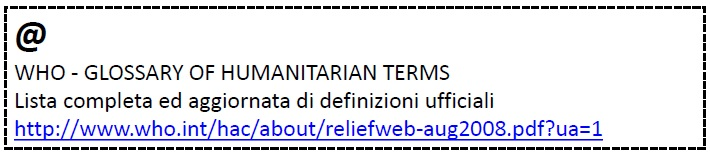
\includegraphics[width=6.58264in,height=4.29167in]{media/image1.jpeg}

Nel \emph{sotterraneo} abbiamo due tipi di falde: la \textbf{falda
freatica} (la prima falda al di sotto della superficie) e poi le
\textbf{falde profonde} che si creano per percolamento dell'acqua
attraverso uno strato solido (l'acqua incontra poi uno strato di terreno
impermeabile come l'argilla, ad esempio, e invece di attraversarlo
scorre anche a notevole distanza).

Le \emph{acque di superficie} possono essere: i \textbf{laghi e bacini
artificiali} (la cui captazione prevede la scelta di punti centrali) i
\textbf{fiumi} (l'acqua è captata a monte dei centri urbani) il
\textbf{mare} (è importante, ma l'acqua non viene utilizzata, sia per la
contaminazione ma soprattutto per la grande salinità e l'alto costo per
abbatterla).

Le \emph{acque meteoriche}: legate alle \textbf{piogge},
approvvigionamento tipico di aree siccitose e con scarse acque nel
sottosuolo che noi ormai non utilizziamo più.

Le acque da destinarsi al consumo umano sono acque trattate o non
trattate, destinate ad uso potabile (come bevanda, pulizie ecc), a
prescindere dalla loro origine e distribuite tramite cisterne o
bottiglie.

DEFINIZIONI

\begin{itemize}
\item
  Acqua di sorgente: attinta direttamente alla fonte, che non è trattata
  né deve essere trattata, naturale, pura allo stato naturale o
  imbottigliata alla sorgente, protetta per natura da ogni pericolo di
  inquinamento e non richiede trattamento di disinfezione, da
  indirizzare all' uso umano; acqua pura che risponde a determinati
  indici, fisici chimici e microbiologici, che devono restare costanti
  nel tempo
\item
  Acqua minerale naturale: le caratteristiche sono quelle dell'acqua di
  sorgente, in più esercita effetti positivi sulla salute, o farmacologi
  o fisiologici
\item
  Acqua termale: acqua naturale usata per scopi terapeutici con
  concentrazione modificata di sali
\item
  Acqua potabile: acqua per consumo umano con requisiti già detti, in
  più possiede caratteristiche più definite di limpidezza, deve essere
  inodore, incolore, senza potenziale danno tossico, biologico e
  chimico, utilizzata dall'uomo (potabile vuol dire che viene resa
  potabile dall'uomo, quindi con bonifica e disinfezione).
\end{itemize}

PROBLEMI PER L'APPROVVIGIONAMENTO (sottosottosezione)

Il problema dell'acqua oggi è l'impoverimento delle fonti di
approvvigionamento.

L' impoverimento si è avuto soprattutto nell'ultimo secolo per:

\begin{itemize}
\item
  Aumentata richiesta dell'uomo per usi personali, per incremento
  demografico
\item
  Attività agricole, zootecniche e industriali intensive, aumentate per
  l'aumento della popolazione
\item
  Urbanizzazione: richieste elevate soprattutto per le qualità della
  vita.
\item
  Incremento dei rifiuti sia solidi sia liquidi che portano ad un
  aumento di contaminazione dell'ambiente e successivamente delle acque,
  così il cerchio si chiude.
\end{itemize}

PROBLEMI DI CONTAMINAZIONE (sottosezione)

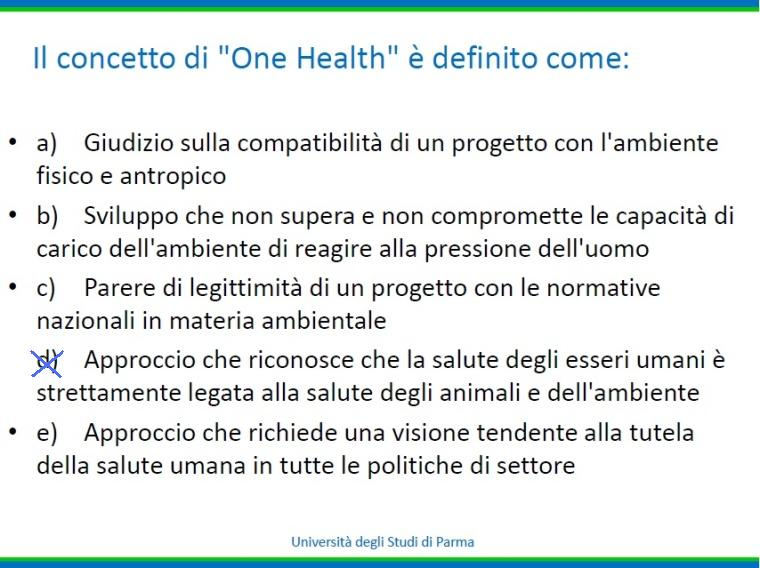
\includegraphics[width=6.69462in,height=4.15663in]{media/image2.jpeg}

\begin{itemize}
\item
  Contaminazione dell'atmosfera: le acque attraversando l'atmosfera si
  caricano di tutto ciò che in essa è presente come pulviscolo, fumi,
  radioattività.
\item
  Contaminazione delle acque di superficie: possono essere inquinate per
  incidenti involontari o per scarichi voluti, industriali e civili, che
  a loro volta percolano del suolo formando le vene superficiali e
  profonde, suscettibili di danno. La contaminazione è ovviamente anche
  dipendente dal suolo, che di per sé riporta inquinanti derivati ad
  esempio da attività agricole come i pesticidi.
\item
  L' apertura incontrollata di pozzi e l'uso di conduzioni non idonee,
  soprattutto quando attraversano lo strato argilloso mettendo in
  comunicazione due falde diverse, pozzi desueti utilizzati come
  discariche ecc.
\item
  Contaminazione del cono alluvionale (per le falde profonde): quando
  partono le fasce di argilla che poi si approfondano in modo vario nel
  suolo e creano le vene, se c'è una costruzione o una attività
  industriale contaminante allora contaminiamo all'origine le falde
  profonde.
\end{itemize}

MATERIALI DI CONTAMINAZIONE (sottosottosezione)

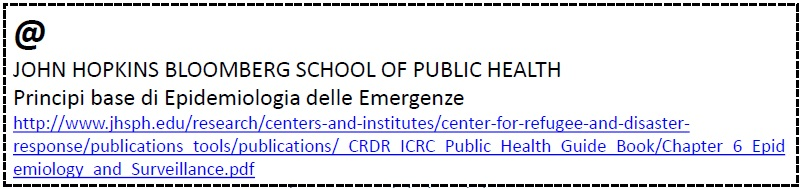
\includegraphics[width=6.69583in,height=4.73681in]{media/image3.jpeg}

Quali sono i materiali di contaminazione?

\begin{itemize}
\item
  reflui industriali organici e non, diretti e indiretti
\item
  scarico di acque calde (inquinamento termico)
\item
  reflui domestici tipicamente biologici, ma non dimenticare i
  detersivi, quindi contaminazione chimica
\item
  reflui agricoli come pesticidi e fertilizzanti
\item
  inquinamento da processi di potabilizzazione, facendo attenzione alle
  tecniche utilizzate e ai materiali chimici
\item
  può essere contaminata anche la rete: per motivi meccanici, in una
  rete che magari non riesce a supportare la dinamica di percorso delle
  strade sovrastanti si ha la creazione di fessurazioni, così l'acqua
  assume inquinanti dall'esterno.
\item
  Ci possono essere difetti delle congiunzioni e difetti del materiale
  delle tubature (esemplare il caso del piombo), la stessa plastica,
  l'acciaio zincato, il cadmio, che possono alterare il pH.
\end{itemize}

Ci sono problemi tecnici di approvvigionamento, di costruzioni, di
manutenzione\ldots{} questo riguarda l'aspetto economico e problemi
anche igienici.

L'acqua deve essere fornita in quantità sufficiente e in qualità
adeguata, deve essere gradevole, priva di rischio biologico e sicura,
priva di sostanze tossiche.

CRITERI DI QUALITÀ (sottosezione)

L'acqua deve rispondere a criteri di qualità desunti e stabiliti a
livello nazionale prendendo atto delle proposte dell'uomo, che si fa
carico di gestire le ricerche e ricavarne le notizie più aggiornate e
utili e tradurle agli stati membri. Dalle proposte dell'OMS vengono
stabilite norme a livello della CEE e poi legiferate in ambito italiano,
prendendo atto di ciò che è stato indicato. Con l'ultimo DDL sulle acque
potabili del 2001 è stato stabilito il valore di parametro di ogni
sostanza affinché l'acqua sia potabile. Questo valore in realtà è
costituito da un \textbf{valore guida}, valore ottimale a cui tendere, e
da un \textbf{valore massimo} che non deve essere superato. Viene
rimandata alla ASL la decisione sulla frequenza con cui vengono fatti i
controlli.

Affinché l'acqua sia considerata igienicamente sicura, cioè potabile,
deve possedere una serie di requisiti: sono i \emph{criteri di
potabilità}.

\begin{itemize}
\item
  IDROGEOLOGICI E LOCALISTICI che riguardano la conoscenza del terreno
  da cui andremo ad attingere acqua, sia superficiali che profonde
\end{itemize}

\begin{itemize}
\item
  ORGANOLETTICI (sapore, odore, colore, limpidezza)
\item
  FISICI (temperatura , pH)
\item
  MICROBIOLOGICI (assenza di patogeni)
\item
  CHIMICI (assenza di sostanze chimiche pericolose per la salute)
\end{itemize}

Dal punto di vista didattico i caratteri CHIMICI vengono divisi in
quattro sottogruppi:

\begin{enumerate}
\def\labelenumi{\arabic{enumi}.}
\item
  Componenti normali (indici di mineralizzazione; l'acqua da bere non
  può essere distillata, deve avere componenti normali che la rendono
  bevibile ed accettabile)
\item
  Componenti che comportano per la loro presenza o quantità problemi di
  usabilità: la durezza, crea problemi di usabilità, con la formazione
  di concrezioni e depositi nei termoriscaldatori, nei pastorizzatori o
  boiler domestici. Non danno problemi di salute, sono prevalentemente
  legati a sali di calcio e magnesio, con una durezza che può essere
  permanente o temporanea (tipo quando bolliamo l'acqua di Parma e la
  pentolina diventa tutta bianca).
\item
  Componenti che recano danno alla salute: il sodio per la correlazione
  con patologie cardiovascolari (ipertensione); il fluoro deve essere
  presente nell'acqua, che ne rappresenta uno dei principali
  apportatori. Se è poco si ha carie dentale, se troppo si ha fluorosi
  dentale. I nitrati portano patologie nel neonato o nell'adulto
  causando ipossia per la formazione di metaemoglobina (nel lattante, a
  causa della flora microbiologica particolare). La componente organica
  parte dall' ammoniaca poi trasformata in nitriti e poi nitrati, che
  possono anche essere di supporto per la crescita di microrganismi.
\item
  Componenti dovuti a contaminazioni (indesiderabili o tossici, ad
  esempio arsenico, vanadio, cadmio, a cui oggi si aggiunge la
  radioattività).
\end{enumerate}

Molto importanti sono inoltre i caratteri MICROBIOLOGICI. L'acqua,
ricevendo scarichi fognari, umani, industriali e agricoli, si può
caricare di microrganismi presenti nell'ambiente e sulle superfici.
Alcuni agenti patogeni opportunisti sono trasmissibili per via idrica ed
emessi principalmente (ma non tutti) con le feci.

\begin{itemize}
\item
  BATTERI (S.tiphi e altre salmonelle, E.coli, Proteus, Serratia spp.,
  Shighella spp., Vibrio colerae, Legionella pn., Listeria m.,
  Campylobacter j\ldots{}.)
\item
  VIRUS (Epatite A E, Enterovirus, Rotavirus, Norovirus, Reovirus,
  Calicivirus\ldots{})
\item
  MICETI
\item
  PROTOZOI ELMINTI (Giardia lamblia, C. Parvum, Entameba
  Histolytica\ldots{})
\end{itemize}

Molti di questi microrganismi sono difficili o impossibili da coltivare
perché hanno bisogno di tempi lunghi; inoltre derivando da scarichi
umani o non umani (abbiamo saltuarietà di emissione) la loro presenza
nell'acqua è molto saltuaria. Abbiamo bisogno di un sistema rapido per
rilevarli, ed è per questo che si utilizza la strada degli INDICATORI
che ci dicono indirettamente se è presente il microrganismo, in modo
semplice, facile e rapido.

1\emph{.Indicatore biologico generale}: di cattiva qualità igienica,
indica la carica batterica. Con temperatura ambientale di 22 gradi o
dell'habitat umano a 36 gradi.

2.\emph{indicatore fecale}, specifico di qualità igienica; primi tra
tutti sono ricercati i coliformi, cioè simili a E. Coli, ma che a
differenza sua vivono nell'ambiente; si ricercano quindi microrganismi
sempre presenti nell'essere umano (E. Coli) e quindi costantemente
eliminati, facilmente individuabili in laboratorio in tempi brevi e
inoltre ci possono fornire informazioni sulla tempistica di
contaminazione. Insieme ai Coliformi totali e ad E. Coli si cercano
anche gli Streptococchi fecali (ex enterococchi) e le spore di C.
Perfringens. Se li ricerchiamo tutti avremo anche un dato di ricchezza
(si può ragionare sulla tempistica), infatti trovare coliformi da soli
significherà che la contaminazione si è realizzata nell'arco di un paio
di settimane, invece gli enterococchi hanno una durata molto inferiore
nell'ambiente esterno (circa una settimana). Il ritrovamento di spore
indica una contaminazione di lunga data, poiché hanno un'emivita molto
lunga. Il valore più importante è quello di E. coli perché è
esclusivamente umano quindi se lo trovo nell'acqua è sicuramente
indicatore di una contaminazione di liquami. I coliformi totali sono
invece presenti anche nell'ambiente e quindi hanno un peso minore. Gli
streptococchi sono anche animali.

Di seguito una tabella indicativa, vedete che il volume utilizzato è
quasi sempre di 100 millilitri.

\begin{longtable}[]{@{}lll@{}}
\toprule
PARAMETRO & CONC MAX & OSSERVAZIONI\tabularnewline
\midrule
\endhead
E.coli & 0/100 ml volume & Limite inderogabile\tabularnewline
Enterococchi & 0/100ml & Limite inderogabile\tabularnewline
Coliformi totali & 0/100ml & Valore condizionato *\tabularnewline
Carica batterica generale a 22◦C & & Valore condizionato*\tabularnewline
\bottomrule
\end{longtable}

La potabilizzazione è la correzione dei caratteri anomali fisici,
organolettici e chimici e anche la disinfezione per la sicurezza
biologica dell'acqua.

MODALITÀ DI CORREZIONE DEI CARATTERI CHIMICO - FISICI INDESIDERATI
(sottosottosezione)

Sono quei caratteri che determinerebbero l'impossibilità di utilizzo
dell'acqua (ad esempio eccesso di torbidità, di colorazione, presenza
eccessiva di Fe, Mn, eccesso di sale).

FILTRI: usati per la torbidità e la colorazione (l'acqua viene
chiarificata tramite flocculazione che fa aderire le sostanze
intorbidanti e la fa sedimentare).

RESINE A SCAMBIO IONICO : per correggere la durezza.

ELETTROOSMOSI, OSMOSI INVERSA, RESINE A SCAMBIO IONICO: utilizzate per
la dissalazione.

Il problema dell'utilizzo dell'acqua salata a livello pratico non
esiste: abbiamo i mezzi per la dissalazione. Sono però processi molto
costosi e, in relazione alla quantità di acqua di cui abbiamo bisogno,
non è conveniente.

MODALITÀ DI CORREZIONE DEI CARATTERI MICROBIOLOGICI = DISINFEZIONE
DELL'ACQUA (sottosottosezione)

Tutte le acque vengono trattate, sono poche le acque profonde che
potrebbero essere già accettabili.

I mezzi più utilizzati per la disinfezione sono quelli chimici che
vedono l'utilizzo di Cloro e di Ozono. Ci sono poi anche metodi fisici.

MEZZI CHIMICI (paragrafo)

\textbf{1) CLORO}: In acqua, sia cloro gas che ipocloriti, formano acido
Ipocloroso (HCLO) che si dissocia in H\textsuperscript{+} e
OCL\textsuperscript{-}; questa reazione è instabile e fortemente
influenzata dal pH: avremo massima possibilità di trovare HCLO in
ambiente acido mentre prevarrà la forma dissociata in ambiente alcalino;
quando è dissociato non è più disinfettante.

\emph{CLORAZIONE SEMPLICE} ci dice semplicemente la quantità minima da
utilizzare per dare cloro residuo (la quantità minima utile alla cloro
richiesta) cioè la quantità che mi certifica che sono state ossidate le
sostanze presenti. Si può determinare con quantità d'acqua stabilita
(100ml) in soluzione con concentrazioni crescenti di cloro e con l'
aggiunta di un indicatore di ossido-riduzione; l'acqua viene lasciata a
contatto con il cloro circa mezz'ora e l'indicatore di ossido-riduzione
ci indica, \emph{col colore giallo,} quando cominciano a comparire
tracce di cloro residuo, cioè quando siamo arrivati al valore soglia,
quando è stata saturata la cloro richiesta. Non so però se il viraggio
derivi da HCLO o dai Cl-composti. In questo la clorazione controllata è
più raffinata.

\emph{CLORAZIONE AL BREAK-POINT O CONTROLLATA}: l'obbiettivo è arrivare
a capire esattamente quando ho avuto un'ossidazione completa, cioè
quando non ho più neanche cloro composti perché anche questi sono stati
ossidati. Mi rimane solo HCLO perché non ho più sostanze organiche,
quindi non ho più cloro richiesta. E' una clorazione calibrata in base
al tipo d'acqua e ci dice quanto cloro aggiungere alla soluzione per
soddisfare la cloro-richiesta.

\textbf{2) OZONO}: potentissimo ossidante, più costoso e meno
maneggevole del cloro, molto veloce nella sua azione senza cattivi odori
nè sapori sgradevoli, è un ottimo processo di disinfezione.

Differenze: il cloro è miscibile in acqua ed ha un effetto residuo nel
tempo, è molto semplice da utilizzare, l'ozono no, quindi devo costruire
degli ozonizzatori (torri di oltre 7 metri) che creano problemi
all'acqua nella circolazione, che obbligano cioè l'acqua ad entrare in
contatto con l'ozono che viene insufflato controcorrente. Come capacità
abbattente sono abbastanza simili.

MEZZI FISICI (paragrafo)

\begin{itemize}
\item
  \textbf{Calore}, obsoleto, però è uno dei migliori mezzi di
  disinfezione di cui disponiamo ad esempio in situazioni difficili tipo
  un terremoto se utilizziamo acqua in quantità minime.
\item
  \textbf{Raggi UV}, potenti ma un grosso limite è il costo ed a scarsa
  resa.
\end{itemize}

GESTIONE DELLE ACQUE (sottosezione)

Passiamo ora alla gestione delle acque o del servizio idrico integrato:

È stato introdotto per realizzare una compattazione verticale di tutti i
gestori del problema acqua: dalla captazione, alla potabilizzazione,
alla distribuzione, al recupero, al trattamento delle acque reflue. Più
attori vengono inglobati in un unico attore in modo da contenere anche i
costi.

Sono escluse le acque industriali e agricole. Il tutto è regolato dalla
Legge Galli del 1994 poi ripreso nel 2006.

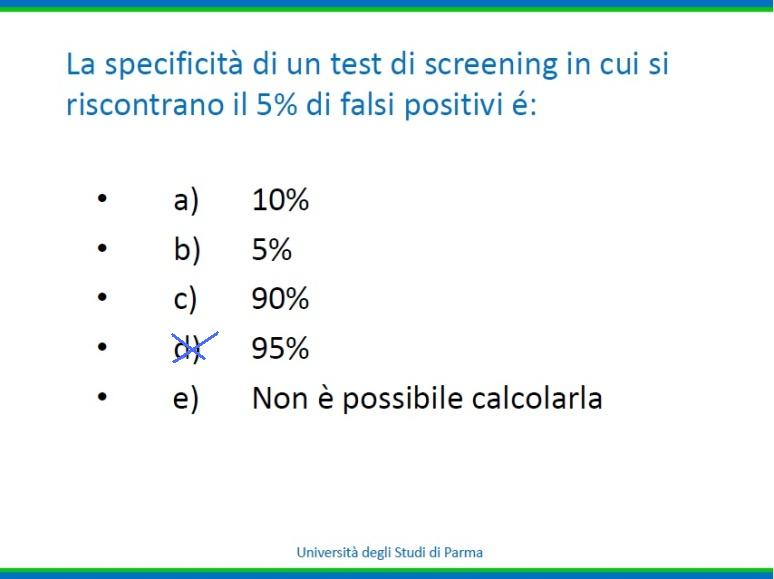
\includegraphics[width=6.69583in,height=3.73494in]{media/image4.jpeg}

In Ambito territoriale abbiamo una organizzazione ottimale in cui
abbiamo un gestore responsabile di tutta la gestione delle acque. La
tariffa viene commisurata ai costi di servizio e agli interventi
necessari per mantenere il servizio. Oggi i gestori funzionanti sono 72.

Attori: in primis i cittadini, il comune può esso stesso gestire o
affidare a un privato la manutenzione, l'erogazione e anche la
distribuzione.

Piano d'ambito: permette di attivare una gestione integrata e un piano
economico e finanziario e la disponibilità economica per attuarlo. Chi
si occupa della manutenzione e modula la tariffa? Ci sono l'acquedotto,
le fogne e la depurazione.

Nel 2011 c'è stato un referendum abrogativo dell'articolo 154 che
dispone che le tariffe del servizio siano determinate tenendo conto
dell'adeguatezza della remunerazione del capitale investito. Nella legge
prima, nella bolletta era previsto un incremento come recupero per
l'investimento del gestore ed è stata abbonata, in modo che venga
provvisto in altro modo.

Quali sono i problemi? In Italia l'aspetto importante è che
nell'acquedotto il 30\% dell'acqua viene persa; da non dimenticare anche
i consumi sbagliati, non solo i problemi di rete: bisognerebbe limitare
le perdite, avere una doppia rete idrica, incentivare le tecnologie che
richiedono una minor quota di acqua a parità di produzione.

RADIAZIONI (sezione)

\textbf{Ionizzanti}: possono produrre ionizzazioni degli atomi dei corpi
che attraversano, con formazione di radicali liberi e procurano un danno
biologico importante. Sono i raggi X, raggi gamma ecc. Sono sia
particelle che onde ad alto contenuto energetico, caricano sia atomi che
molecole dopo la rottura dei legami atomici. La capacità di penetrazione
dipende dal tipo e dallo spessore del mezzo attraversato e dalla
tipologia di radiazione e dalla quantità di radiazioni.

\begin{enumerate}
\def\labelenumi{\arabic{enumi}.}
\item
  Radiazioni alfa: con grande capacità ionizzante e limitata capacità di
  diffusione nell'aria.
\item
  Radiazioni beta: elettroni più penetranti delle alfa
\item
  Radiazioni gamma: con eccitazione del nucleo ed elevata capacità
  penetrante.
\end{enumerate}

Normativa: in Italia il rischio dell'impiego delle radiazioni è regolato
dal decreto legislativo 295. Dal 2007 c'è un nuovo decreto che
disciplina la gestione delle sorgenti radioattive ad alta attività.

\textbf{Gas}: \emph{radon} presente nelle abitazioni con effetto
cancerogeno ed importante fattore di rischio per il tumore al polmone.
Deriva dal terreno, viene emesso dal suolo e da materiali di
costruzione. È un gas nobile inerte, a partenza dall' uranio ma
sostanzialmente deriva dal radio come ultima fase di decadimento.
Prevenzione: spazi areati, depressurizzazione dei locali, aumento dei
ricambi d'aria, sigillazione delle fessurazioni, mappatura delle zone a
rischio.

\textbf{Campi elettromagnetici}: sono campi derivati dal movimento di
correnti elettriche e tali oscillazioni producono campi elettromagnetici
diffusi tramite onde, che sono una forma di propagazione di energia e si
propagano anche nel vuoto con velocità di 300 mila km al secondo. Ogni
onda ha una sua frequenza in hertz, maggior frequenza vuol dire maggiore
energia trasportata. L'insieme di tutte le onde è classificata in base
alla frequenza ed è lo spettro delle onde, diviso in base alla capacità
di ionizzare la materia.

Come detto prima le radiazioni possono essere ionizzanti e non.
L'inquinamento è dato dalle radiazioni non ionizzanti.

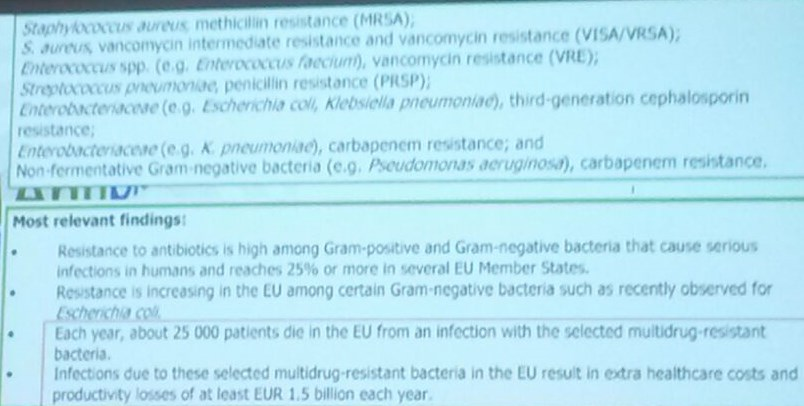
\includegraphics[width=6.69583in,height=4.71181in]{media/image5.jpeg}

Effetto biologico: variazioni fisiologiche in un organo o un sistema;
l'effetto biologico principale è la produzione di correnti elettriche
sovrapposte a quelle naturali che portano a sovraeccitazioni nervose.

Danno alla salute vuol dire perdita di salute. Quali sono i danni?

Acuti o cronici.

\begin{enumerate}
\def\labelenumi{\arabic{enumi}.}
\item
  Acuti per esposizione massiva al di sopra di una soglia di
  compensazione in ambito lavorativo
\item
  Cronici per sommatoria di effetti su basse concentrazioni ma per
  periodi abbastanza lunghi, c'è un aumento dell'esposizione e un
  aumento delle possibilità di contrarre un danno la cui qualità non
  cambia se il danno si presenta.
\end{enumerate}

Esposizione ad alte frequenze: causano opacizzazione del cristallino,
anomalie della cornea, alterazione delle funzioni muscolari neurali

Esposizioni a bassa frequenza: hanno effetti sulla vista, sul snc,
stimolazione dei tessuti eccitabili con extrasistoli, fibrillazione
ventricolare.

L'IARC ha decretato come `possibile' effetto delle radiazioni sulla
salute la cancerogenicità in esposizione ad elevati livelli
residenziali, ma non in esposizione professionale.

La normativa italiana disciplina in modo diverso l'esposizione alle alte
e basse frequenze con un decreto che riguarda tutti gli impianti, i
sistemi, le apparecchiature per usi civili e militari che possono
esporre la popolazione a campi tra 0 e 300 GigaHertz.

INQUINAMENTO ACUSTICO (sezione)

Concentrazione del rumore a seconda delle zone residenziali più o meno
protette, si fa una valutazione notturna e diurna con definizione dei
valori limite ammissibili per classe. Ha incidenza notevole sulla
qualità di vita.

AMIANTO (sezione)

Molto utilizzato negli anni `80 nelle costruzioni perché ignifugo, i
corpi asbestosi sono potenziali cancerogeni data la loro dimensione, con
predisposizione al tumore ai polmoni e al mesotelioma pleurico. La legge
ne ha infatti imposto il divieto di utilizzo.

RIFIUTI LIQUIDI (sezione)

Un aspetto importante della gestione del sistema idrico integrato è la
gestione dei rifiuti liquidi.

Problematiche:

\begin{itemize}
\item
  Infettive: per la presenza nei rifiuti stessi di virus, batteri
\item
  Tossiche: per la potenziale presenza di sostanze tossiche
\item
  Danno estetico per l'ambiente: cattivo odore, colorazione delle acque,
  schiumeggiamento
\item
  Economiche: liquami non correttamente smaltiti causano difficoltà di
  recupero di acque inquinanti, con conseguente perdita di acqua per uso
  umano, ma anche per attività ricreative come ad esempio il nuoto o la
  pesca oppure per uso agricolo.
\end{itemize}

Possiamo fare una suddivisione per tipologia dei liquami:

\begin{itemize}
\item
  Liquami organici: derivanti da feci, urine, pulizie, dalla cottura di
  alimenti con una carica microbica imponente data dai commensali del
  nostro intestino insieme ad eventuali patogeni
\item
  Acque industriali: una parte è identica ai liquami civili, a questa si
  aggiungono acque usate per i processi industriali ad esempio di
  raffreddamento, con aggiuntivo inquinamento termico.
\item
  Rifiuti speciali: derivanti da attività mediche come ospedali, studi
  odontoiatrici, istituto di ricerca, con una loro normativa di
  smaltimento (smaltite in modo diverso a seconda della sostanza
  contaminante).
\end{itemize}

Il primo passo è quello di allontanare i liquami dalle nostre case.
Come?

Tramite sistemi di fognatura, in passato prettamente statiche, oggi
dinamiche con sistemi unitari con un'unica rete di controllo di liquami
e acque bianche, oppure un sistema separato di sistemi di canalizzazione
o un sistema misto che le prevede entrambe, ma sempre dinamico.

SCHEMA DI TRATTAMENTO (sottosezione)

I liquami non possono essere immessi tout court nell'ambiente:

\begin{enumerate}
\def\labelenumi{\arabic{enumi}.}
\item
  abbiamo una fase di \emph{pre-trattamento}, o processo primario : una
  sgrossatura che consiste nella grigliatura cioè far passare il liquame
  attraverso delle griglie a maglie sempre più strette per allontanare
  materiale grossolano; oltre alla grigliatura vi sono anche la
  dissabbiatura e la sgrassatura
\item
  \begin{quote}
  \emph{Processo secondario}: attraverso filtri percolatori prevede la
  separazione delle parti più colloidali con formazione di un eloato
  chiarificato e di fanghi secondari.
  \end{quote}
\item
  \emph{Trattamento terziario}: per l'eloato chiarificato si ha un
  ulteriore abbattimento ed eventualmente disinfezione prima di essere
  immessi nell'ambiente e possono essere usati come fertilizzanti.
\end{enumerate}

\end{document}
